\documentclass[10pt]{article}
\usepackage[utf8]{inputenc}
\usepackage[shortlabels]{enumitem}
\usepackage[margin=1in]{geometry}
\usepackage{setspace}
\usepackage{hyperref}
\usepackage{graphicx}
\onehalfspacing
\setlength{\parskip}{1em}
\setlength{\parindent}{0pt}
\bibliographystyle{ecta}
\usepackage[T1]{fontenc}
\usepackage{titling}
\usepackage{amsmath}
\setlength{\droptitle}{-7em}
\addtolength\abovedisplayskip{-3in}
\addtolength\belowdisplayskip{-3in}

\title{City Location Choice and Household Productivity}
\preauthor{}
\postauthor{}
\author{Tan Sein Jone}
\predate{}
\postdate{}
\date{}
%\Today

\begin{document}
\doublespacing
\maketitle

\section{Introduction}

The location choice of households is an important determinant of the spatial distribution of economic activity. The choice of location is influenced by a variety of factors such as the availability of jobs, the cost of living, and the quality of public services. In this paper, I develop a model of city location choice that incorporates the productivity of households as an important determinant of location choice. I show that the productivity of households is an important determinant of the spatial distribution of economic activity and that it can help explain the observed patterns of urbanization.

The model is based on the idea that households are more productive in cities because of the agglomeration of economic activity. In particular, households are more productive in certain cities due to the presence of occupations that are complementary to their skills. For example, a household with skills in finance may be more productive in a city with a large financial sector. Similarly, a household with skills in technology may be more productive in a city with a large technology sector. The model shows that households choose to locate in cities where they are most productive, leading to the agglomeration of economic activity in certain cities.

This leads to two key outcomes. First, larger cities will tend to have higher levels of economic activity because they are able to attract more households. Second, cities that specialize in specific occupations will tend to be more attratcive to households with those skills. This leads to the agglomeration of economic activity in cities that specialize in specific occupations.

We achieve this by developing a model of city location choice that is based on Quantitative Spacial Models develoepd by Redding (2016) which loads city heterogeneity onto a city ammenity term in order to avoid a trivial solution of all hosueholds choosing to live in once city. This model however comes comes with the independence of irrelavent alternatives (IIA) assumption, which makes cities perfect substitutes for each other. We relax this assumption by using a nested CES structure with correlation proposed by Lind and Ramondo (2023) to allow for correlated draws of productivity between cities, making cities imperfect substitutes for each other.

Both of these models are based off the class of discrete choice models proposed by Eaton and Kortum (2002) which determines production shares of different goods by taking probabalistic draws of productivity of different countries. Rather than having these productivities determine prices, we will draaw productivities for households which determine wages and hence utility across different cities.

\subsection{Literature Review}

\section{Model of Production}

\begin{align}
    Y_{c} (\nu) = \prod_k Q_{ck} (\nu)^{\omega_{ck}}
\end{align}

Consider a closed economy consisting of $N$ cities and a continuim of hosuehold types $\nu \in [0, 1]$. Each city $c$ employs hosueholds of type $\nu$ in occupation $k$ to produce output $Y_{ck} (\nu)$ using a Cobb-Douglas production function with technology $Z_{ck} (\nu)$. We assume no trade costs between cities, and that the price of goodproduced by occupation $k$ is freely traded and priced under perfect competition.

The price index of city $c$ is $\Phi_c$. The wage of a hosuehold in occupation $k$ in city $c$ is $w_{ck} (\nu) = \Phi_c Z_{ck} (\nu)$. We asusme that when a hosuehold chooses to work in a particular occupation $k$, they will be randomly allocated to a sector within a given city. As in EK, productivity is a random variable drawn from a max stable mutivariate Fr\'{e}chet distribution and is dependent on both the city and the occupation. Output produced by a specific occuaption is also assumed to be produced by a random sector.

\begin{align}
    U (\nu) = \max_c \left\{ \Phi_c Z_{ck} (\nu) \right\}
\end{align}

A hosuehold's utility is purely determined by wages and is given by the maximum wage across all cities. We assume that hosueholds are risk neutral and hence maximize expected utility. When choosing a prticular city to maximize utility, households will simultaneously choose an occupation to work in. We assume that hosueholds are perfectly mobile and can move to any city at no cost.

\section{Max Stable Multivariate Fr\'{e}chet Distribution}

\begin{align}
    P[Z_{1k}(\nu) < z, \dots, Z_{Nk}(\nu) < z] = \exp \left\{ \left[ - \sum_{c}^{N} (T_{ck} H_k(\nu) z^{- \theta})^{\frac{1}{1 - \rho_k}} \right]^{1 - \rho_k} \right\}
\end{align}

We assume that productivity is distributed max stable multivariate Fr\'{e}chet where $T_{ck}$ is the scale parameter for city $c$ and occupation $k$. $H_k(\nu)$ is the occupation specific productivity shifter for household of type $\nu$ in occupation $k$. The heterogeneity of this shifter reflects the difference in human capital across different hosuehold types. $\theta > 0$ is the shape parameter, characterizing the tail behaviour of the distribution. $\rho_k$ is the occupation specific correlation parameter, which dictates the extent to which productivity draws are correlated acorss cities for occupation $k$.

\begin{align}
    T_{ck} = T_c T_k t_{ck}
\end{align}

Looking at the scale parameter $T_{ck}$, we can separate it into three components. $T_c$ is the city specific scale parameter which captures the attractiveness of a city, shifting the distribution for all productivity draws within that city. $T_k$ is the occupation specific scale parameter which is common across all cities, this captures the aggregate effect that occupation $k$ has on productivity. An example shock to this parameter is the effect new computers have on an occupation that heavily relies on computation. $t_{ck}$ is the city-occupation specific scale paramter which captures the idiosyncratic effect of city $c$ on occupation $k$. The effect on new york on finance is an example of this.

\begin{align}
    Z_c(\nu) = \max_k \left\{ Z_{ck} (\nu) \right\}
\end{align}

A household's schedule of productivities is characterized by a vector of draws from diferent fr\'{e}chet distributions for each city occupaiton pair. The realized productivity of a household of type $\nu$ has in city $c$ is the occupation that maximizes the productivity that particular hosuehold has in the city.

\begin{align}
    P[Z_1(\nu) < z, \dots, Z_N(\nu) < z] = \exp \left\{ - \sum_{k}^{} \left[ \sum_{c}^{N} (T_c H(\nu) z^{- \theta})^{\frac{1}{1 - \rho_k}} \right]^{1 - \rho_k} \right\}
\end{align}

Unlike sequential games where households might pick a city before picking an occupation, we assume that households pick both simultaneously. This is because thhe schedule of productivity already determines the ideal occupation of a household in a city. From here, we can obatin the joint distribution of all productivities being less than some value $z$ for all cities and occupations.

\begin{align}
    Z(\nu) = \max_c \left\{ \frac{Z_c (\nu)}{\Phi_c} \right\}
\end{align}

The joint probability takes on the form of a max stable multivariate Fr\'{e}chet distribution with a cross-nested CES correlation structure as proposed by Lind and Ramondo (2023). This distribution is a generalization of the Fr\'{e}chet distribution to the multivariate case, and is used to model the joint distribution of extreme values. This is similar to the GEV distribution, but with the added flexibility of allowing for correlation between the draws of different cities across occupations. A household of type $\nu$ has the realized productivity that is hence characterized by the maximum of all productivity draws across all cities and occupations scaled by the inverse of that city's price index $\Phi_c$.

\subsection{Correlation Function}

\begin{align}
    P[Z_1 < z, \dots, Z_N < z] = \exp \left\{ - \sum_{k}^{} \left[ \sum_{c}^{N} (T_c z^{- \theta})^{\frac{1}{1 - \rho_k}} \right]^{1 - \rho_k} \right\}
\end{align}

When we intergrate over all hosuehold types for a particular hosuehold shifter, we get the average productivity shifter for that occupation which we assume to be 1 for all occupations $\int_{0}^{1} H_k (\nu) d\nu = 1$. With the case of a corss-nested CES function, we can approximate a correlation function. Assuming that productivity is distributed max-stable multivariate Fr\'{e}chet, with scale parameter $T_{ck}$ shape parameter $\theta$ and correlation parameters $\rho_k$.

\begin{align}
    G(Z_1^{- \theta}, \dots, Z_N^{- \theta}) = \sum_{c}^{N} T_{ck} z^{- \theta}
    \label{ces}
\end{align}

\begin{align}
    G(Z_1^{- \theta}, \dots, Z_N^{- \theta}) = \sum_{k}^{} \left[ \sum_{c}^{N} (T_{ck} z^{- \theta})^{\frac{1}{1 - \rho_k}} \right]^{1 - \rho_k}
    \label{nested_ces}
\end{align}

Where $Z_c^{- \theta} = (\gamma \Phi_c)^{- \theta}$ and $\gamma = \Gamma \left( \frac{\theta - 1}{\theta} \right)$. $\Gamma(\cdot)$ is the gamma function. Expression~\ref{ces} shows the standard Fr\'{e}chet distribution with independent productivity in which the strength of comparative advantage is solely governed by th shape parameter $\theta$. Once we abandon this assumption as in Lind and Ramondo (2023), we can obtain a correlation function that allows for correlated draws of productivity across cities as in expression~\ref{nested_ces}. When here exists only one occupation, the correlation parameter will be 0 and expression~\ref{nested_ces} will reduce to expression~\ref{ces}.

\subsection{Choice Shares}

\begin{align}
    \pi_c = \frac{Z_c^{- \theta} G_c(Z_1^{- \theta}, \dots, Z_N^{- \theta})}{G(Z_1^{- \theta}, \dots, Z_N^{- \theta})}
\end{align}

The expression above gives us the city specific choice shares of hosueholds. Where $G_c(Z_1^{- \theta}, \dots, Z_N^{- \theta}) = \partial G(Z_1^{- \theta}, \dots, Z_N^{- \theta}) / \partial Z_c^{- \theta}$. In order to evaluate this expression, we make this simplifying assumption that the correlation parameter is the same across all occupations $\rho_k = \rho$. This allows us to obtain the following expression for the choice shares.

\begin{align}
    \pi_{c} = (Z_{c}^{-\theta})^{\frac{1}{1-\rho}}\Bigg[\frac{\sum\limits_{k}{T^{\frac{1}{1-\rho}}_{ck}}\lambda_{k}^{-\rho}}{\sum\limits_{k}\lambda_{k}^{1-\rho}}\Bigg]
    \label{city_shares}
\end{align}

We define $\lambda_k = \sum\limits_{c}^{N}{T^{\frac{1}{1-\rho}}_{ck}}(Z_{c}^{-\theta})^{\frac{1}{1-\rho}}$. $Z_c^{- \theta}$ simply acts as a city level shifter that scales the productivity of all hosueholds in that city. The second term in brackets is a measure of a city $c$'s relative strength across occupations. As any individual $T_{ck}$ increases, the share of that that city also increases. Conversely, as the strength of other cities in a given occupation $\lambda_k$ increases, the share of that city decreases. This is because the city is less attractive relative to other cities in that occupation.

\begin{align}
    \pi_{ck} = \frac{Z_c^{- \theta} G_c^k(Z_1^{- \theta}, \dots, Z_N^{- \theta})}{G^k(Z_1^{- \theta}, \dots, Z_N^{- \theta})}
\end{align}

\begin{align}
    \pi_{ck} = \frac{(T_{ck} Z_c^{-\theta})^{\frac{1}{1 - \rho_k}}}{\sum_{c}^{N} (T_{ck} Z_c^{-\theta})^{\frac{1}{1 - \rho_k}}}
    \label{city_occuaption_shares}
\end{align}

$G^k (Z_1^{-\theta}, \dots, Z_N^{-\theta}) = [\sum_{c}^{N} (T_{ck} Z_c^{-\theta})^{\frac{1}{1 - \rho_k}}]^{1 - \rho_k}$ is the occupation specific function that allows us to evaluate the city specific share of occupaitons. In this case, we can can abandon the simplifying assumption of $\rho_k = \rho$ and obtain the expression for the choice shares of cities within a gievn occupation. This share is simply teh share of productivities relative to all other city's productivities within a given occupation. Notice that as that occupation becomes more correlated across cities, the relative strength of that city starts to matter more.

\subsection{Cross and Within City Elasticities}

\begin{align}
    \epsilon_{cck} = \frac{\partial \ln \pi_{ck}}{\partial \ln T_{ck}} \approx \frac{1}{1 - \rho} \phi_{ck} > 0
\end{align}

\begin{align}
    \phi_{ck} = \frac{T_{ck}^{\frac{1}{1 - \rho}} \lambda_k^{- \rho}}{\sum_{k}^{} T_{ck}^{\frac{1}{1 - \rho}} \lambda_k^{- \rho}}
\end{align}

We approximate this derivative by assuming that each city is small and therefore $\partial \ln \lambda_k / \partial \ln T_{ck} \approx 0$. This allows us to obtain the expression for the elasticity of a city's own price. Notice that a city's own price elasticity is positive, and increasing in the relavance of a given occupation for a gievn city. That is, as $T_{ck}$ increases, the elasticity increases. If a gievn city is particularly productive in occuaption $k$, then changes in $T_{ck}$ will have an outsized effect on that city's overall choice share. Put it another way: becoming more productive in occupations for which you are already everyone's last choice will not do much to alter the overall choice share of your city. $\phi_{ck}$ captures the extent to which this city is relatively more productive at occupation $k$ than other cities compared to all other cities in every occupaiton.

\begin{align}
    \epsilon_{cc'k} = \frac{\partial \ln \pi_{ck}}{\partial \ln T_{c'k}} \approx - \pi_{c'} \phi_{c'k} \left[ 1 + \left( \frac{\rho}{1 - \rho} \right) \left( \frac{\phi_{ck}}{\omega_k} \right) \right] < 0
\end{align}

\begin{align}
    \omega_k = \frac{\lambda_k^{1 - \rho}}{\sum_{k}^{} \lambda_k^{1 - \rho}}
\end{align}

We can approximate the cross-price elasticity in a similar fashion. The first term in this derivative simply captures the "CES" element: if city $c'$ is large and has a particularly string comparative advantage in occupaiton $k$, then technology shocks in this city-occupation pair will have large effects elsewhere. This is captured by the size $\pi_{c'k}$ and the comparative advantage $\phi_{c'k}$.

The second term captures the unbalanced substitution patterns associated with correlated choice probabilities. Notice first that if $\rho = 0$, this model is simple CES in substitution patterns. As $\rho \to 1$, the correlated choices dominate the CES element more and more. City $c$ will be particularly effected by shocks to city $c'$ in occupation $k$ is city $c$ is also productive in occupation $k$. In fact, it is the multiple of $\phi_{c'k} \phi_{ck}$ that dictates the strength of substitution.

But why is this substitution dampened by weight $\omega_k$? Notice that is occupation $k$ is very attractive and $\omega_k \to 1$, this implies that there are many attractive cities for households productive in occupation $k$. That is, we cannot determine the cross-price elasticity without considering the environment in which both $c$ and $c'$ exist, and the strength of substitution between them is strongest when they are both productive in $k$ and no other cities are even close, implying a small $\omega_k$.

\begin{align}
    \epsilon_{ckck} = \frac{\partial \ln \pi_{ck}}{\partial \ln T_{ck}} = \frac{1}{1 - \rho_k} \left[ 1 - \pi_{ck} \right] > 0
\end{align}

\begin{align}
    \epsilon_{ckc'k} = \frac{\partial \ln \pi_{ck}}{\partial \ln T_{c'k}} = - \frac{1}{1 - \rho_k} \pi_{c'k} < 0
\end{align}

Elasticities within occupations can similarly be derived, this time without any approximaitons. Notice that both the within and corss-price elasticities are scaled by the $\frac{1}{1 - \rho_k}$ parameter, with both increasing as $\rho_k$ increases. This means that as occupations become more correlated across cities, the elasticities increases. For the second term in the within price elasticity, as $\pi_{ck}$ increases, the elasticity decreases. This illustrates a diminishing returns effect where cities with high levels of city-occuaption choice shares will have lower returns for any increases in productivity. In other words, when a city has a high level of choice shares in a given occupation, it has less to gain from further increases in productivity in that occupation relative to teh shares it already has.

The opposite is true for cross-price elasticities, where the higher levels of $\pi_{c'k}$ will increase the elasticity. This is because the more productive a city is in a given occupation, the more it will be affect another city's choice shares within that given occupation. $\pi_{c'k}$ neatly illustrates the gravity effect where large cities have larger effects on other cities.

\section{Simulations}

\begin{table}[h]
    \centering
    \begin{tabular}{|l|c|c|c|}
        \hline
                          & \textbf{Detriot} & \textbf{Chicago} & \textbf{New York} \\
        \hline
        \textbf{Trades}   & 7                & 8                & 3                 \\
        \hline
        \textbf{Services} & 2                & 1                & 8                 \\
        \hline
    \end{tabular}
    \caption{City Scale Parameters $T_{ck}$}
    \label{city_shifter}
\end{table}

Assume now that we have two occupations, trades and services. We will also assuem three cities, Detriot, Chicago and New York with Detriot and Chicago specializing in trades and New York specializing in services. Thehe scale parameters for each city-occupation pair are as shown in Table \ref{city_shifter}. The correlation parameter $\rho_k$ is set to 0.7 for services and 0.5 for trades and the shape paramter is set to 2.

For each hosuehold, they will draw a $K \times N$ matrix of productivities from specific Fr\'{e}chet distributions where $K$ is the number of occupations and $N$ is the number of cities. The realized productivity of hosueholds is then the maximum productivity across all cities and occupations. The column index of this productivity determines the city at which the household chooses to locate, and the row index determines the occupation that the household chooses to work in. This will give us our choice shares for each city and occupation.

\begin{figure}[!htb]
    \begin{minipage}{0.5\textwidth}
        \centering
        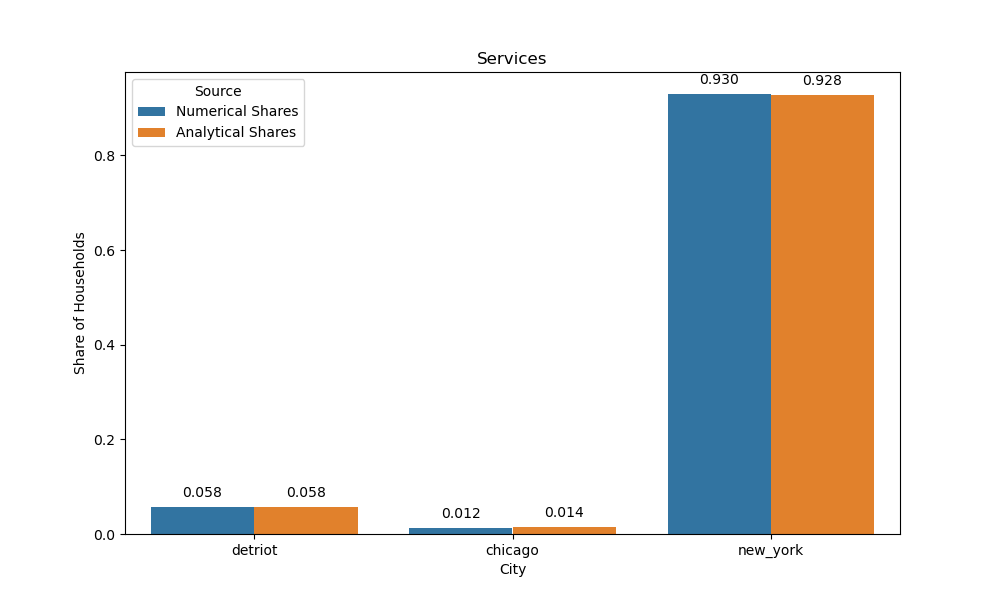
\includegraphics[width=\textwidth]{../../simulations/graphs/sim_services.png}
        \caption{Service Choice Shares}
        \label{sim_services}
    \end{minipage}
    \begin{minipage}{0.5\textwidth}
        \centering
        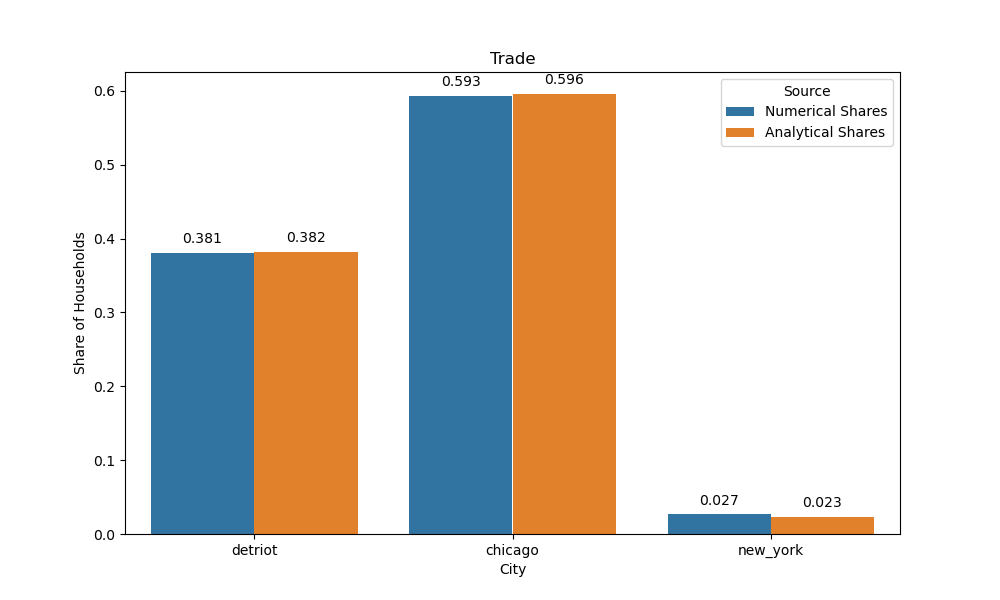
\includegraphics[width=\textwidth]{../../simulations/graphs/sim_trade.png}
        \caption{Trades Choice Shares}
        \label{sim_trades}
    \end{minipage}
\end{figure}

\begin{figure}[!htb]
    \centering
    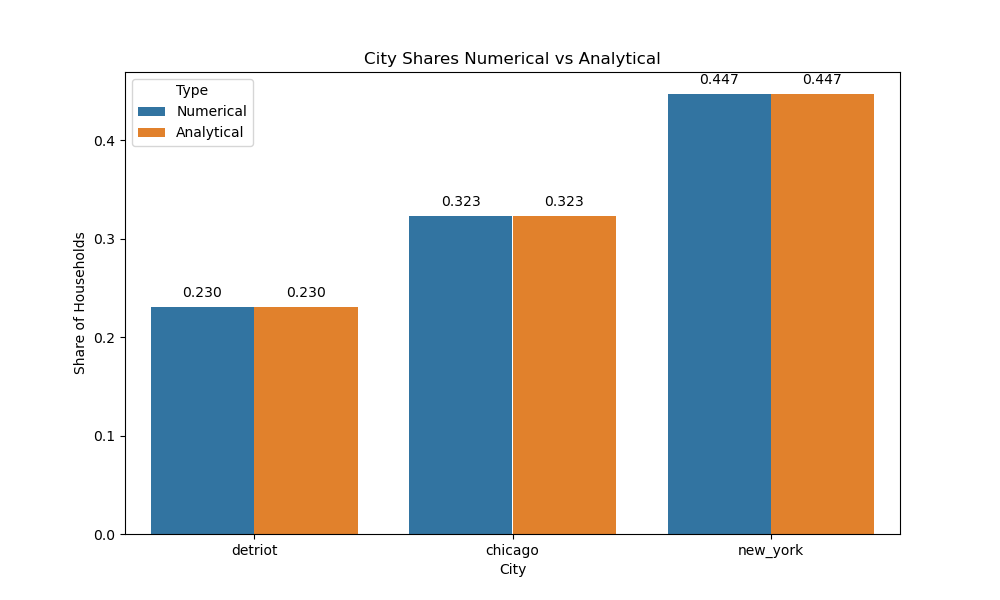
\includegraphics[width=\textwidth]{../../simulations/graphs/sim_city_shares.png}
    \caption{City Choice Shares}
    \label{sim_city_shares}
\end{figure}

We now draw 10000 hosuheolds, simulating the distribution of location choice shares across cities and occuations. This numerical solution will now be compared to our analytical solution for choice shares as discussed in the previous section. Figure \ref{sim_services} and Figure \ref{sim_trades} show the simulated occupation specific choice shares for services and trades respectively. The analytical solution is given by expression~\ref{city_occuaption_shares}. The same excercise is repeated for city choice shares as shown in Figure \ref{sim_city_shares}. Expression~\ref{city_shares} gives us the analytical solution for city choice shares. Consistent with our simplifying assumption, $\rho_k = \rho$ for all and it is assumed to be the average of our two $\rho_k$ values. The numerical results closely match the analytical results, validating our analytical solution.

\begin{figure}[!htb]
    \begin{minipage}{0.5\textwidth}
        \centering
        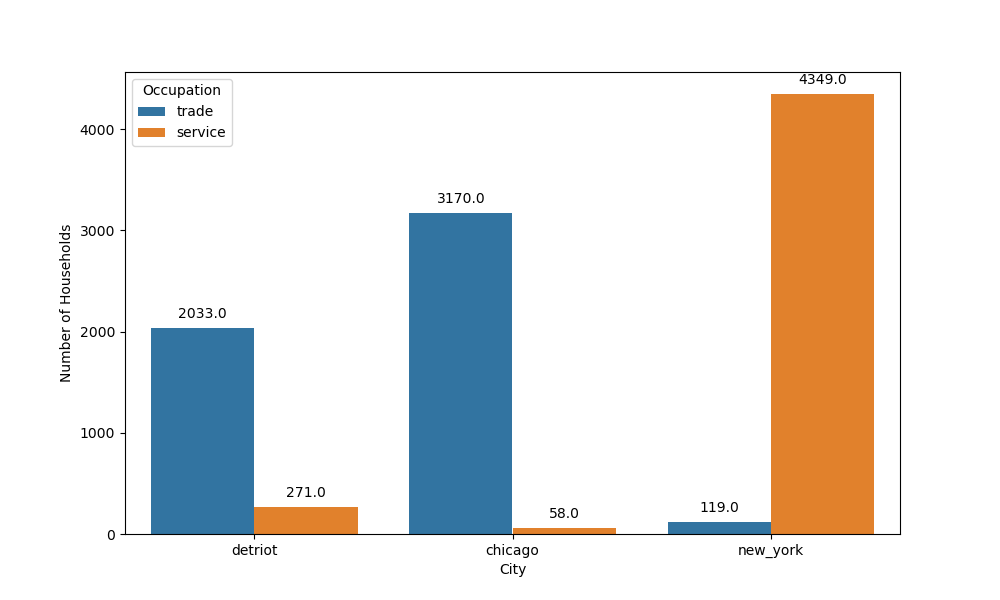
\includegraphics[width=\textwidth]{../../simulations/graphs/city_pop.png}
        \caption{Initial City Population}
        \label{city_pop}
    \end{minipage}
    \begin{minipage}{0.5\textwidth}
        \centering
        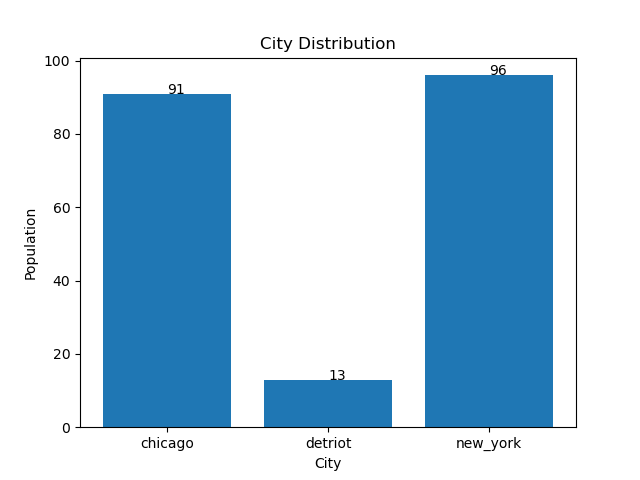
\includegraphics[width=\textwidth]{../../simulations/graphs/c_shock.png}
        \caption{Post Detriot Shock City Population}
        \label{c_shock}
    \end{minipage}
\end{figure}

Now that our analytical solutions have been verified, we will now begin to examine the behaviour of our model to ensure it's consistency with intitial intuitions. Figure \ref{city_pop} shows the initial population distribution across cities. New York has the highest population due to it being the only city specializing in services with Detriot and Chicago sharing trades focused hosuheolds. The slight bias towards Chicago is expected due to it's higher scale parameter for trades. We will now shock Detriot's trades scale parameter by 0.5 times it's original value and observe the change in city populations. As shown in Figure \ref{c_shock}, the population of Detriot decreases significantly, with Chicago and New York increasing in population. AS expected, the majority of the households working in trades have relocated to Chicago, with some moving to New York. New York meanwhile picks up the majority of households working in services from Detriot. This is consistent with our intuitions that households working in specific occupations will move to cities that specialize in those occupations.

\end{document}